\section{Simulation and Data Sample}

The method by which all of the measurements presented in this thesis are done is that of \emph{Monte-Carlo (MC) forward folding}. In a nutshell, this method involves producing a large set of simulated signal and background events that are then re-weighted in such a way that their distribution matches that of the observed data events as closely as possible. In order to give reliable results, an accurate simulation of all the particle interactions described in section~\ref{sec:particle-interactions} as well as the detector electronics described in section~\ref{sec:dom-daq} is required. Both simulated and observed events are then passed through the same data processing chain described in section~\ref{sec:data-processing}. The resulting MC simulated dataset and the observed dataset are then histogrammed in the same binning, and the weights of the MC events are adjusted to give the best match between the histograms according to a loss function as defined in section~\ref{sec:test-statistic}.

The simulation chain for neutrinos and atmospheric muons can generally be divided into three steps that are described in this chapter:
\begin{enumerate}
    \item Simulation of particle interactions
    \item Photon propagation in ice
    \item Response of detector DAQ systems
\end{enumerate}
A special case is the simulation of detector noise, for which no particle production or photon propagation is necessary.

\subsection{Particle Interactions}

The first step for the simulation of neutrinos and muons is to sample parameters for the primary particle, and to simulate the secondary charged particles that are produced when it interacts inside the detector. The charged components of the secondary particles are then passed on to the photon propagation step described in section~\ref{sec:photon-propagation}.

\subsubsection{Neutrinos}

Because of the inherently low interaction rate of neutrinos, it would be impractical to simulate a constant flux of neutrinos from any particular direction, the vast majority of which would simply pass through the detector without producing any signal at all. Instead, every simulated neutrino is forced to interact within a given volume, and the event is given a weight corresponding to the inverse of the simulated fluence,
\begin{equation}
    w = \frac{1}{F_{\mathrm{sim}}} \frac{1}{N_{\mathrm{sim}}}\;,
\end{equation}
where $N_{\mathrm{sim}}$ is the number of simulated events and $F_{\mathrm{sim}}$ is the fluence per area, solid angle, energy, and time. This weight, when multiplied with the flux of a given physics model and a live time, gives the expected number of events that this simulated event corresponds to.
%% TODO: I'm honestly not sure if it is necessary to explicitly calculate the start- and endpoints and calculate the length of the path through the cylinder. In my mind, if the position is randomly chosen inside the volume, then the weight should also only depend on the volume. The path taken through the volume should only matter if absorption plays a role
%For this analysis, the simulated interaction volume is a cylinder centered in DeepCore, with a length and radius chosen such that all events that have a chance of producing a signal in DeepCore should be contained in it. The neutrino directions are sampled isotropically in azimuth and zenith, implying that the simulated flux per solid angle is $\phi_\Omega = \frac{1}{4\pi}$. The simulated neutrino flux is a power law with $\phi_e \propto E^{-2}$. After sampling the zenith and azimuth for an event, a random position is sampled  
Under the assumption that neutrino absorption is negligible and that the material consists of isoscalar targets, the simulated fluence is given by the chosen probability density in the direction and energy, $\phi_\Omega \times \phi_E$,  the size of the interaction volume, $V$, the cross-section of the interaction, $\sigma$, and the density of the material, $\rho$, by
\begin{equation}
    F_{\mathrm{sim}}^{-1} = V \times \rho \times N_A \times 1\frac{\mathrm{mol}}{\mathrm{g}} \times \sigma \times \frac{1}{\phi_\Omega} \times \frac{1}{\phi_E}\;,
\end{equation}
where $N_A$ is Avogadro's number. The volume in which neutrino interactions are simulated is a cylinder centered in DeepCore, with a length and radius chosen such that all events that have a chance of producing a signal in DeepCore should be contained in it, depending on the neutrino flavor and energy (see also table~\ref{table:GENIE}). Neutrino directions are isotropically distributed in zenith and azimuth, implying $\phi_\Omega = \frac{1}{4\pi}$. The neutrino energies are sampled from a power law with $\phi_e \propto E^{-2}$. The simulated live time corresponding to a single simulated event is  $T_{\mathrm{sim}} =  F_{\mathrm{sim}} / \Phi$, where $\Phi$ is the expected neutrino flux including neutrino oscillations at global best-fit parameters. The amount of simulation generated for each neutrino flavor is chosen such that the total simulated live time is $\sim 70$~years. Neutrinos and anti-neutrinos are produced in ratios of 70\% and 30\%, respectively. The simulated live time as a function of energy is shown in figure~\ref{fig:sim-livetime}. The livetime for electron neutrinos is increasing with energy because the simulated spectrum is harder than the real spectrum. The livetime for tau neutrinos is much higher than that of other flavors because the contribution of tau neutrinos to the expected neutrino flux is very small.

\begin{table}
\caption{Table of generation volumes used for \textsc{Genie} neutrino simulation. The cylinder is centered in DeepCore in all cases. \label{table:GENIE}}
\begin{center}
\begin{tabular}{ ccccc } 
\textbf{Flavor} & \textbf{Energy (GeV)} & \textbf{Radius (m)} & \textbf{Length (m)}\\
\toprule
\multirow{4}{*}{$\nu_e+\bar{\nu_e}$}  & 1-4 & 250 & 500 \\
 & 4-12 & 250 & 500   \\ 
 & 12-100 & 350 & 600  \\
 & 100-10000 & 550 & 1000  \\
 \midrule
\multirow{4}{*}{$\nu_{\mu}+\bar{\nu_{\mu}}$} & 1-5 & 250 & 500\\
 & 5-80 & 400 & 900\\
 & 80-1000 & 450 & 1500\\
 & 1000-10000 & 550 & 1500\\
 \midrule
\multirow{5}{*}{$\nu_{\tau}+\bar{\nu_{\tau}}$} & 1-4 & 250 & 500\\
 & 4-10 & 250 & 500\\
 & 10-50 & 350 & 600\\
 & 50-1000 & 450 & 800\\
 & 1000-10000 & 550 & 1500\\
 \bottomrule
\end{tabular}
\end{center}
\end{table}

\begin{figure}
    \centering
    
\tikzsetnextfilename{mc_livetime}%
\begin{tikzpicture}

\pgfplotstableread{figures/icecube/selection/livetime/livetime_hists.csv}\table

\begin{loglogaxis}[
    width=0.7\linewidth,
    height=0.5\linewidth,
    tick align=outside,
    tick pos=left,
    xmin=1, xmax=10000,
    xmajorgrids,
    ymajorgrids,
    xlabel=energy (GeV),
    ylabel=total MC livetime (years),
    ymin=20, ymax=80000,
    legend style={
      at={(0.95,0.95)},
      anchor=north east,
    },
]
% livetimes in the table are months per file
% number of files taken from the nominal MC only
\addplot[const plot, black, thick] table[x=energy, y expr=613 * \thisrow{genie_120000} / 12] from \table;
\addlegendentry{\(\nu_e\)}
\addplot[const plot, orange, thick] table[x=energy, y expr=1519 * \thisrow{genie_140000} / 12]  from \table;
\addlegendentry{\(\nu_\mu\)}
\addplot[const plot, skyblue, thick] table[x=energy, y expr=340 * \thisrow{genie_160000} / 12]  from \table;
\addlegendentry{\(\nu_\tau\)}
\end{loglogaxis}

\end{tikzpicture}

    \caption{Simulated livetime for per file, calculated using the HKKM model flux with \textsc{NuFit}~2.2\cite{nufit22} oscillation parameters.}
    \label{fig:sim-livetime}
\end{figure}

After sampling the parameters of the primary neutrino, the \textsc{Genie}~\sidecite{Andreopoulos:2015wxa} software is used to simulate its interaction with the ice and the production of secondary particles and to calculate the cross-section of the interaction. The propagation and Cherenkov light production of any muon that is produced in these interactions is simulated with \textsc{Proposal}\sidecite{proposal}. 

\subsubsection{Atmospheric muons}

\subsection{Photon Propagation}
\label{sec:photon-propagation}

\subsection{Simulation of Detector Response}

\subsection{Final Sample and Binning}
\label{sec:sample-binning}
The starting point for this analysis is a DeepCore data sample consisting of 7.5 years of good live time and 21,914 events that pass through all selection steps described in section~\ref{sec:data-processing}. For every event in the sample, the energy and zenith angle is reconstructed as discussed in section~\ref{sec:event-reconstruction}. Both data and simulation sets are binned in reconstructed energy ($E_{\rm reco}$), cosine of the reconstructed zenith angle ($\cos(\theta_z)$), and PID as follows:

\begin{itemize}
    \item $E_{\rm reco}$: 11 bins spanning the range from 6.31~GeV to 158.49~GeV, the two bins with the highest energy are merged.
    \item $\cos(\theta_z)$: 10 bins spanning the range from -1 to 0.1
    \item PID: One bin between 0.55 and 0.75, and one bin between 0.75 and 1.0.
\end{itemize}

The lower PID bin between 0.55 and 0.75 consists to 69\%  (pre-fit MC estimate) of charged-current $\nu_\mu + \bar{\nu}_\mu$ events and is referred to as the \emph{mixed} channel, while the higher PID channel between 0.75 and 1.0 consists to 94\% of charged-current $\nu_\mu + \bar{\nu}_\mu$ events and is referred to as the \emph{tracks} channel. The histogram of both channels at the null hypothesis (i.e. no sterile signal) is shown in figure~\ref{fig:nominal-hist-null-hypo}.

\begin{figure}
    \centering
    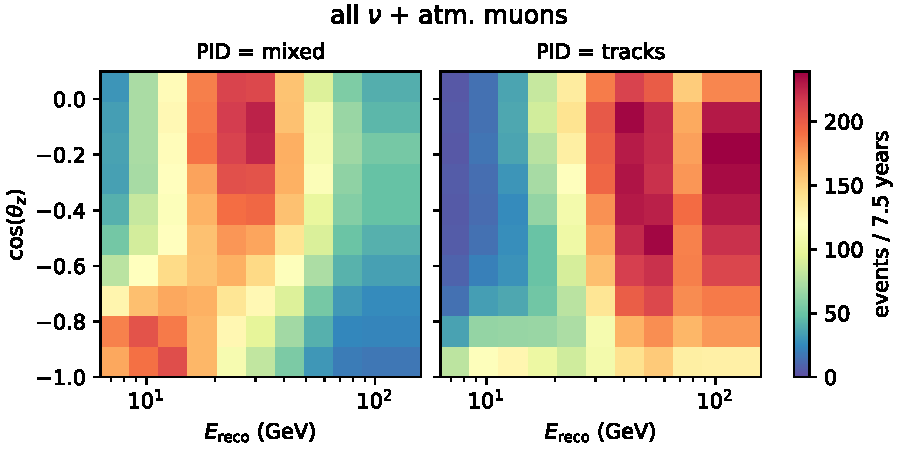
\includegraphics[width=0.8\textwidth]{figures/measurement/simulation_and_data/binning/plot_maps_total.pdf}
    \caption{Expected event counts in 7.5 years of live time assuming no sterile mixing and NuFit~4.0~\cite{nufit40} global best fit parameters at Normal Ordering.}
    \label{fig:nominal-hist-null-hypo}
\end{figure}

\begin{table}[htb]
\centering
\caption{Expected event rate with 8 years livetime broken down in event types and PID bins, calculated at NuFit~4.0 global best fit parameters.}
\label{tab:event-rate}
\begin{tabular}{lccc} \toprule
\hline
Type  & PID & Counts [8 years] & Rate [$\mathrm{\mu Hz}$] \\ \hline
All MC & mixed  &   11428 &   48.3\\
All MC & tracks &   12238 &   51.7\\ \hline
${\nu_{\rm all}} + {\bar\nu_{\rm all}} \, {\rm NC} $ & mixed  &     943 &    4.0 \\
${\nu_e} + {\bar\nu_e} \, {\rm CC}                 $ & mixed  &    1704 &    7.2 \\
${\nu_\mu} + {\bar\nu_\mu} \, {\rm CC}             $ & mixed  &    7901 &   33.4 \\
${\nu_\tau} + {\bar\nu_\tau} \, {\rm CC}           $ & mixed  &     470 &    2.0 \\
muons                                                & mixed  &     410 &    1.7 \\
\hline
${\nu_{\rm all}} + {\bar\nu_{\rm all}} \, {\rm NC} $ & tracks &     171 &    0.7 \\
${\nu_e} + {\bar\nu_e} \, {\rm CC}                 $ & tracks &     294 &    1.2 \\
${\nu_\mu} + {\bar\nu_\mu} \, {\rm CC}             $ & tracks &   11517 &   48.7 \\
${\nu_\tau} + {\bar\nu_\tau} \, {\rm CC}           $ & tracks &     162 &    0.7 \\
muons                                                & tracks &      93 &    0.4 \\
\hline
\hline
\end{tabular}
\end{table}
